\documentclass[1p]{elsarticle_modified}
%\bibliographystyle{elsarticle-num}

%\usepackage[colorlinks]{hyperref}
%\usepackage{abbrmath_seonhwa} %\Abb, \Ascr, \Acal ,\Abf, \Afrak
\usepackage{amsfonts}
\usepackage{amssymb}
\usepackage{amsmath}
\usepackage{amsthm}
\usepackage{scalefnt}
\usepackage{amsbsy}
\usepackage{kotex}
\usepackage{caption}
\usepackage{subfig}
\usepackage{color}
\usepackage{graphicx}
\usepackage{xcolor} %% white, black, red, green, blue, cyan, magenta, yellow
\usepackage{float}
\usepackage{setspace}
\usepackage{hyperref}

\usepackage{tikz}
\usetikzlibrary{arrows}

\usepackage{multirow}
\usepackage{array} % fixed length table
\usepackage{hhline}

%%%%%%%%%%%%%%%%%%%%%
\makeatletter
\renewcommand*\env@matrix[1][\arraystretch]{%
	\edef\arraystretch{#1}%
	\hskip -\arraycolsep
	\let\@ifnextchar\new@ifnextchar
	\array{*\c@MaxMatrixCols c}}
\makeatother %https://tex.stackexchange.com/questions/14071/how-can-i-increase-the-line-spacing-in-a-matrix
%%%%%%%%%%%%%%%

\usepackage[normalem]{ulem}

\newcommand{\msout}[1]{\ifmmode\text{\sout{\ensuremath{#1}}}\else\sout{#1}\fi}
%SOURCE: \msout is \stkout macro in https://tex.stackexchange.com/questions/20609/strikeout-in-math-mode

\newcommand{\cancel}[1]{
	\ifmmode
	{\color{red}\msout{#1}}
	\else
	{\color{red}\sout{#1}}
	\fi
}

\newcommand{\add}[1]{
	{\color{blue}\uwave{#1}}
}

\newcommand{\replace}[2]{
	\ifmmode
	{\color{red}\msout{#1}}{\color{blue}\uwave{#2}}
	\else
	{\color{red}\sout{#1}}{\color{blue}\uwave{#2}}
	\fi
}

\newcommand{\Sol}{\mathcal{S}} %segment
\newcommand{\D}{D} %diagram
\newcommand{\A}{\mathcal{A}} %arc


%%%%%%%%%%%%%%%%%%%%%%%%%%%%%5 test

\def\sl{\operatorname{\textup{SL}}(2,\Cbb)}
\def\psl{\operatorname{\textup{PSL}}(2,\Cbb)}
\def\quan{\mkern 1mu \triangleright \mkern 1mu}

\theoremstyle{definition}
\newtheorem{thm}{Theorem}[section]
\newtheorem{prop}[thm]{Proposition}
\newtheorem{lem}[thm]{Lemma}
\newtheorem{ques}[thm]{Question}
\newtheorem{cor}[thm]{Corollary}
\newtheorem{defn}[thm]{Definition}
\newtheorem{exam}[thm]{Example}
\newtheorem{rmk}[thm]{Remark}
\newtheorem{alg}[thm]{Algorithm}

\newcommand{\I}{\sqrt{-1}}
\begin{document}

%\begin{frontmatter}
%
%\title{Boundary parabolic representations of knots up to 8 crossings}
%
%%% Group authors per affiliation:
%\author{Yunhi Cho} 
%\address{Department of Mathematics, University of Seoul, Seoul, Korea}
%\ead{yhcho@uos.ac.kr}
%
%
%\author{Seonhwa Kim} %\fnref{s_kim}}
%\address{Center for Geometry and Physics, Institute for Basic Science, Pohang, 37673, Korea}
%\ead{ryeona17@ibs.re.kr}
%
%\author{Hyuk Kim}
%\address{Department of Mathematical Sciences, Seoul National University, Seoul 08826, Korea}
%\ead{hyukkim@snu.ac.kr}
%
%\author{Seokbeom Yoon}
%\address{Department of Mathematical Sciences, Seoul National University, Seoul, 08826,  Korea}
%\ead{sbyoon15@snu.ac.kr}
%
%\begin{abstract}
%We find all boundary parabolic representation of knots up to 8 crossings.
%
%\end{abstract}
%\begin{keyword}
%    \MSC[2010] 57M25 
%\end{keyword}
%
%\end{frontmatter}

%\linenumbers
%\tableofcontents
%
\newcommand\colored[1]{\textcolor{white}{\rule[-0.35ex]{0.8em}{1.4ex}}\kern-0.8em\color{red} #1}%
%\newcommand\colored[1]{\textcolor{white}{ #1}\kern-2.17ex	\textcolor{white}{ #1}\kern-1.81ex	\textcolor{white}{ #1}\kern-2.15ex\color{red}#1	}

{\Large $\underline{12a_{1038}~(K12a_{1038})}$}

\setlength{\tabcolsep}{10pt}
\renewcommand{\arraystretch}{1.6}
\vspace{1cm}\begin{tabular}{m{100pt}>{\centering\arraybackslash}m{274pt}}
\multirow{5}{120pt}{
	\centering
	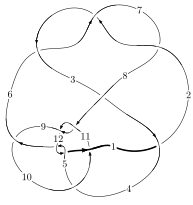
\includegraphics[width=112pt]{../../../GIT/diagram.site/Diagrams/png/1839_12a_1038.png}\\
\ \ \ A knot diagram\footnotemark}&
\allowdisplaybreaks
\textbf{Linearized knot diagam} \\
\cline{2-2}
 &
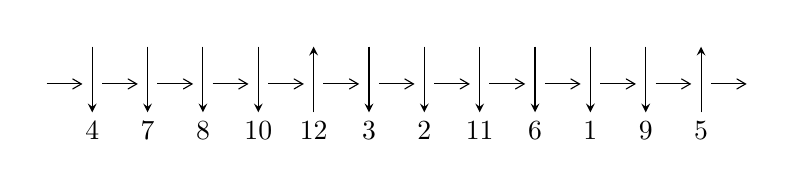
\begin{tikzpicture}[x=20pt, y=17pt]
	% nodes
	\node (C0) at (0, 0) {};
	\node (C1) at (1, 0) {};
	\node (C1U) at (1, +1) {};
	\node (C1D) at (1, -1) {4};

	\node (C2) at (2, 0) {};
	\node (C2U) at (2, +1) {};
	\node (C2D) at (2, -1) {7};

	\node (C3) at (3, 0) {};
	\node (C3U) at (3, +1) {};
	\node (C3D) at (3, -1) {8};

	\node (C4) at (4, 0) {};
	\node (C4U) at (4, +1) {};
	\node (C4D) at (4, -1) {10};

	\node (C5) at (5, 0) {};
	\node (C5U) at (5, +1) {};
	\node (C5D) at (5, -1) {12};

	\node (C6) at (6, 0) {};
	\node (C6U) at (6, +1) {};
	\node (C6D) at (6, -1) {3};

	\node (C7) at (7, 0) {};
	\node (C7U) at (7, +1) {};
	\node (C7D) at (7, -1) {2};

	\node (C8) at (8, 0) {};
	\node (C8U) at (8, +1) {};
	\node (C8D) at (8, -1) {11};

	\node (C9) at (9, 0) {};
	\node (C9U) at (9, +1) {};
	\node (C9D) at (9, -1) {6};

	\node (C10) at (10, 0) {};
	\node (C10U) at (10, +1) {};
	\node (C10D) at (10, -1) {1};

	\node (C11) at (11, 0) {};
	\node (C11U) at (11, +1) {};
	\node (C11D) at (11, -1) {9};

	\node (C12) at (12, 0) {};
	\node (C12U) at (12, +1) {};
	\node (C12D) at (12, -1) {5};
	\node (C13) at (13, 0) {};

	% arrows
	\draw[->,>={angle 60}]
	(C0) edge (C1) (C1) edge (C2) (C2) edge (C3) (C3) edge (C4) (C4) edge (C5) (C5) edge (C6) (C6) edge (C7) (C7) edge (C8) (C8) edge (C9) (C9) edge (C10) (C10) edge (C11) (C11) edge (C12) (C12) edge (C13) ;	\draw[->,>=stealth]
	(C1U) edge (C1D) (C2U) edge (C2D) (C3U) edge (C3D) (C4U) edge (C4D) (C5D) edge (C5U) (C6U) edge (C6D) (C7U) edge (C7D) (C8U) edge (C8D) (C9U) edge (C9D) (C10U) edge (C10D) (C11U) edge (C11D) (C12D) edge (C12U) ;
	\end{tikzpicture} \\
\hhline{~~} \\& 
\textbf{Solving Sequence} \\ \cline{2-2} 
 &
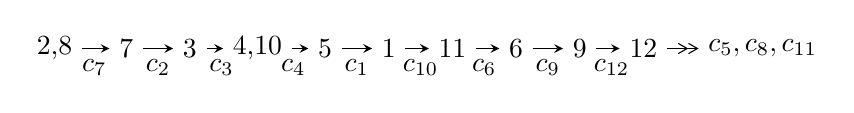
\begin{tikzpicture}[x=23pt, y=7pt]
	% node
	\node (A0) at (-1/8, 0) {2,8};
	\node (A1) at (1, 0) {7};
	\node (A2) at (2, 0) {3};
	\node (A3) at (49/16, 0) {4,10};
	\node (A4) at (33/8, 0) {5};
	\node (A5) at (41/8, 0) {1};
	\node (A6) at (49/8, 0) {11};
	\node (A7) at (57/8, 0) {6};
	\node (A8) at (65/8, 0) {9};
	\node (A9) at (73/8, 0) {12};
	\node (C1) at (1/2, -1) {$c_{7}$};
	\node (C2) at (3/2, -1) {$c_{2}$};
	\node (C3) at (5/2, -1) {$c_{3}$};
	\node (C4) at (29/8, -1) {$c_{4}$};
	\node (C5) at (37/8, -1) {$c_{1}$};
	\node (C6) at (45/8, -1) {$c_{10}$};
	\node (C7) at (53/8, -1) {$c_{6}$};
	\node (C8) at (61/8, -1) {$c_{9}$};
	\node (C9) at (69/8, -1) {$c_{12}$};
	\node (A10) at (11, 0) {$c_{5},c_{8},c_{11}$};

	% edge
	\draw[->,>=stealth]	
	(A0) edge (A1) (A1) edge (A2) (A2) edge (A3) (A3) edge (A4) (A4) edge (A5) (A5) edge (A6) (A6) edge (A7) (A7) edge (A8) (A8) edge (A9) ;
	\draw[->>,>={angle 60}]	
	(A9) edge (A10);
\end{tikzpicture} \\ 

\end{tabular} \\

\footnotetext{
The image of knot diagram is generated by the software ``\textbf{Draw programme}" developed by Andrew Bartholomew(\url{http://www.layer8.co.uk/maths/draw/index.htm\#Running-draw}), where we modified some parts for our purpose(\url{https://github.com/CATsTAILs/LinksPainter}).
}\phantom \\ \newline 
\centering \textbf{Ideals for irreducible components\footnotemark of $X_{\text{par}}$} 
 
\begin{align*}
I^u_{1}&=\langle 
-3.62076\times10^{53} u^{97}+8.81180\times10^{53} u^{96}+\cdots+8.81449\times10^{53} b+4.33084\times10^{53},\\
\phantom{I^u_{1}}&\phantom{= \langle  }1.67240\times10^{54} u^{97}-4.07185\times10^{54} u^{96}+\cdots+8.81449\times10^{53} a-2.98740\times10^{54},\;u^{98}-3 u^{97}+\cdots-5 u+1\rangle \\
\\
\end{align*}
\raggedright * 1 irreducible components of $\dim_{\mathbb{C}}=0$, with total 98 representations.\\
\footnotetext{All coefficients of polynomials are rational numbers. But the coefficients are sometimes approximated in decimal forms when there is not enough margin.}
\newpage
\renewcommand{\arraystretch}{1}
\centering \section*{I. $I^u_{1}= \langle -3.62\times10^{53} u^{97}+8.81\times10^{53} u^{96}+\cdots+8.81\times10^{53} b+4.33\times10^{53},\;1.67\times10^{54} u^{97}-4.07\times10^{54} u^{96}+\cdots+8.81\times10^{53} a-2.99\times10^{54},\;u^{98}-3 u^{97}+\cdots-5 u+1 \rangle$}
\flushleft \textbf{(i) Arc colorings}\\
\begin{tabular}{m{7pt} m{180pt} m{7pt} m{180pt} }
\flushright $a_{2}=$&$\begin{pmatrix}0\\u\end{pmatrix}$ \\
\flushright $a_{8}=$&$\begin{pmatrix}1\\0\end{pmatrix}$ \\
\flushright $a_{7}=$&$\begin{pmatrix}1\\- u^2\end{pmatrix}$ \\
\flushright $a_{3}=$&$\begin{pmatrix}- u\\u^3+u\end{pmatrix}$ \\
\flushright $a_{4}=$&$\begin{pmatrix}- u^3-2 u\\u^3+u\end{pmatrix}$ \\
\flushright $a_{10}=$&$\begin{pmatrix}-1.89733 u^{97}+4.61949 u^{96}+\cdots-13.1123 u+3.38919\\0.410774 u^{97}-0.999695 u^{96}+\cdots+4.99129 u-0.491331\end{pmatrix}$ \\
\flushright $a_{5}=$&$\begin{pmatrix}0.222953 u^{97}-1.13842 u^{96}+\cdots+1.53433 u-1.07411\\0.475801 u^{97}-1.08428 u^{96}+\cdots+1.54473 u-0.514952\end{pmatrix}$ \\
\flushright $a_{1}=$&$\begin{pmatrix}u^7+4 u^5+4 u^3\\- u^7-3 u^5-2 u^3+u\end{pmatrix}$ \\
\flushright $a_{11}=$&$\begin{pmatrix}-0.469168 u^{97}+0.658638 u^{96}+\cdots-3.66130 u+1.52455\\-0.262625 u^{97}+0.897029 u^{96}+\cdots-3.81810 u+1.84336\end{pmatrix}$ \\
\flushright $a_{6}=$&$\begin{pmatrix}u^2+1\\- u^4-2 u^2\end{pmatrix}$ \\
\flushright $a_{9}=$&$\begin{pmatrix}-0.484597 u^{97}+0.957708 u^{96}+\cdots-6.36097 u+3.14188\\-0.393812 u^{97}+1.22529 u^{96}+\cdots-4.19603 u+1.78580\end{pmatrix}$ \\
\flushright $a_{12}=$&$\begin{pmatrix}0.00745162 u^{97}-0.615653 u^{96}+\cdots+4.96278 u-2.02379\\0.381053 u^{97}-0.953602 u^{96}+\cdots+0.502513 u+0.295011\end{pmatrix}$\\&\end{tabular}
\flushleft \textbf{(ii) Obstruction class $= -1$}\\~\\
\flushleft \textbf{(iii) Cusp Shapes $= 1.63646 u^{97}-5.49263 u^{96}+\cdots+8.71271 u-12.4499$}\\~\\
\newpage\renewcommand{\arraystretch}{1}
\flushleft \textbf{(iv) u-Polynomials at the component}\newline \\
\begin{tabular}{m{50pt}|m{274pt}}
Crossings & \hspace{64pt}u-Polynomials at each crossing \\
\hline $$\begin{aligned}c_{1}\end{aligned}$$&$\begin{aligned}
&u^{98}-19 u^{97}+\cdots-841339 u+59603
\end{aligned}$\\
\hline $$\begin{aligned}c_{2},c_{6},c_{7}\end{aligned}$$&$\begin{aligned}
&u^{98}+3 u^{97}+\cdots+5 u+1
\end{aligned}$\\
\hline $$\begin{aligned}c_{3}\end{aligned}$$&$\begin{aligned}
&u^{98}-3 u^{97}+\cdots+595 u+425
\end{aligned}$\\
\hline $$\begin{aligned}c_{4}\end{aligned}$$&$\begin{aligned}
&u^{98}- u^{97}+\cdots- u-1
\end{aligned}$\\
\hline $$\begin{aligned}c_{5},c_{12}\end{aligned}$$&$\begin{aligned}
&u^{98}-3 u^{97}+\cdots+u+1
\end{aligned}$\\
\hline $$\begin{aligned}c_{8},c_{11}\end{aligned}$$&$\begin{aligned}
&u^{98}- u^{97}+\cdots-33 u-1
\end{aligned}$\\
\hline $$\begin{aligned}c_{9}\end{aligned}$$&$\begin{aligned}
&u^{98}+5 u^{97}+\cdots-3041767 u-195991
\end{aligned}$\\
\hline $$\begin{aligned}c_{10}\end{aligned}$$&$\begin{aligned}
&u^{98}+9 u^{97}+\cdots+4943 u-137
\end{aligned}$\\
\hline
\end{tabular}\\~\\
\newpage\renewcommand{\arraystretch}{1}
\flushleft \textbf{(v) Riley Polynomials at the component}\newline \\
\begin{tabular}{m{50pt}|m{274pt}}
Crossings & \hspace{64pt}Riley Polynomials at each crossing \\
\hline $$\begin{aligned}c_{1}\end{aligned}$$&$\begin{aligned}
&y^{98}+45 y^{97}+\cdots+84576889997 y+3552517609
\end{aligned}$\\
\hline $$\begin{aligned}c_{2},c_{6},c_{7}\end{aligned}$$&$\begin{aligned}
&y^{98}+89 y^{97}+\cdots-7 y+1
\end{aligned}$\\
\hline $$\begin{aligned}c_{3}\end{aligned}$$&$\begin{aligned}
&y^{98}+13 y^{97}+\cdots+6423025 y+180625
\end{aligned}$\\
\hline $$\begin{aligned}c_{4}\end{aligned}$$&$\begin{aligned}
&y^{98}-3 y^{97}+\cdots-99 y+1
\end{aligned}$\\
\hline $$\begin{aligned}c_{5},c_{12}\end{aligned}$$&$\begin{aligned}
&y^{98}+73 y^{97}+\cdots-7 y+1
\end{aligned}$\\
\hline $$\begin{aligned}c_{8},c_{11}\end{aligned}$$&$\begin{aligned}
&y^{98}-67 y^{97}+\cdots-179 y+1
\end{aligned}$\\
\hline $$\begin{aligned}c_{9}\end{aligned}$$&$\begin{aligned}
&y^{98}-203 y^{97}+\cdots-3248967720299 y+38412472081
\end{aligned}$\\
\hline $$\begin{aligned}c_{10}\end{aligned}$$&$\begin{aligned}
&y^{98}+137 y^{97}+\cdots-6924923 y+18769
\end{aligned}$\\
\hline
\end{tabular}\\~\\
\newpage\flushleft \textbf{(vi) Complex Volumes and Cusp Shapes}
$$\begin{array}{c|c|c}  
\text{Solutions to }I^u_{1}& \I (\text{vol} + \sqrt{-1}CS) & \text{Cusp shape}\\
 \hline 
\begin{aligned}
u &= \phantom{-}0.065339 + 1.097010 I \\
a &= -1.324380 - 0.441285 I \\
b &= \phantom{-}1.46093 + 1.29019 I\end{aligned}
 & -4.40512 - 2.11265 I & \phantom{-0.000000 } 0 \\ \hline\begin{aligned}
u &= \phantom{-}0.065339 - 1.097010 I \\
a &= -1.324380 + 0.441285 I \\
b &= \phantom{-}1.46093 - 1.29019 I\end{aligned}
 & -4.40512 + 2.11265 I & \phantom{-0.000000 } 0 \\ \hline\begin{aligned}
u &= \phantom{-}0.612404 + 0.652469 I \\
a &= -0.252396 - 0.753912 I \\
b &= -0.216088 + 0.660826 I\end{aligned}
 & -3.29048 - 3.02837 I & \phantom{-0.000000 } 0 \\ \hline\begin{aligned}
u &= \phantom{-}0.612404 - 0.652469 I \\
a &= -0.252396 + 0.753912 I \\
b &= -0.216088 - 0.660826 I\end{aligned}
 & -3.29048 + 3.02837 I & \phantom{-0.000000 } 0 \\ \hline\begin{aligned}
u &= \phantom{-}0.800888 + 0.357291 I \\
a &= \phantom{-}0.253454 + 0.756910 I \\
b &= \phantom{-}0.106025 - 0.595292 I\end{aligned}
 & -4.30667 - 1.74398 I & \phantom{-0.000000 } 0 \\ \hline\begin{aligned}
u &= \phantom{-}0.800888 - 0.357291 I \\
a &= \phantom{-}0.253454 - 0.756910 I \\
b &= \phantom{-}0.106025 + 0.595292 I\end{aligned}
 & -4.30667 + 1.74398 I & \phantom{-0.000000 } 0 \\ \hline\begin{aligned}
u &= -0.038346 + 1.161800 I \\
a &= -1.262120 - 0.527027 I \\
b &= \phantom{-}0.316673 - 1.090610 I\end{aligned}
 & -0.080038 + 0.981236 I & \phantom{-0.000000 } 0 \\ \hline\begin{aligned}
u &= -0.038346 - 1.161800 I \\
a &= -1.262120 + 0.527027 I \\
b &= \phantom{-}0.316673 + 1.090610 I\end{aligned}
 & -0.080038 - 0.981236 I & \phantom{-0.000000 } 0 \\ \hline\begin{aligned}
u &= -0.468868 + 0.684398 I \\
a &= -1.050430 - 0.676356 I \\
b &= \phantom{-}1.047240 - 0.388987 I\end{aligned}
 & \phantom{-}0.46550 - 4.30305 I & -7.01592 + 4.36620 I \\ \hline\begin{aligned}
u &= -0.468868 - 0.684398 I \\
a &= -1.050430 + 0.676356 I \\
b &= \phantom{-}1.047240 + 0.388987 I\end{aligned}
 & \phantom{-}0.46550 + 4.30305 I & -7.01592 - 4.36620 I\\
 \hline 
 \end{array}$$\newpage$$\begin{array}{c|c|c}  
\text{Solutions to }I^u_{1}& \I (\text{vol} + \sqrt{-1}CS) & \text{Cusp shape}\\
 \hline 
\begin{aligned}
u &= \phantom{-}0.820805\phantom{ +0.000000I} \\
a &= -0.384972\phantom{ +0.000000I} \\
b &= -0.00973519\phantom{ +0.000000I}\end{aligned}
 & -4.50628\phantom{ +0.000000I} & -26.0090\phantom{ +0.000000I} \\ \hline\begin{aligned}
u &= \phantom{-}0.486220 + 0.652272 I \\
a &= -2.00701 + 0.85445 I \\
b &= \phantom{-}1.61190 + 0.78207 I\end{aligned}
 & -4.55395 + 9.86790 I & -10.03674 - 4.17482 I \\ \hline\begin{aligned}
u &= \phantom{-}0.486220 - 0.652272 I \\
a &= -2.00701 - 0.85445 I \\
b &= \phantom{-}1.61190 - 0.78207 I\end{aligned}
 & -4.55395 - 9.86790 I & -10.03674 + 4.17482 I \\ \hline\begin{aligned}
u &= -0.741511 + 0.323631 I \\
a &= -1.21304 - 1.63056 I \\
b &= \phantom{-}1.42634 + 0.75096 I\end{aligned}
 & -0.79939 + 8.54144 I & -9.35248 - 8.62618 I \\ \hline\begin{aligned}
u &= -0.741511 - 0.323631 I \\
a &= -1.21304 + 1.63056 I \\
b &= \phantom{-}1.42634 - 0.75096 I\end{aligned}
 & -0.79939 - 8.54144 I & -9.35248 + 8.62618 I \\ \hline\begin{aligned}
u &= -0.154621 + 1.182450 I \\
a &= \phantom{-}0.442376 + 0.325025 I \\
b &= -0.24214 - 1.49177 I\end{aligned}
 & -0.62174 + 5.21555 I & \phantom{-0.000000 } 0 \\ \hline\begin{aligned}
u &= -0.154621 - 1.182450 I \\
a &= \phantom{-}0.442376 - 0.325025 I \\
b &= -0.24214 + 1.49177 I\end{aligned}
 & -0.62174 - 5.21555 I & \phantom{-0.000000 } 0 \\ \hline\begin{aligned}
u &= \phantom{-}0.734303 + 0.335173 I \\
a &= -1.56251 + 2.65545 I \\
b &= \phantom{-}1.95978 - 1.35725 I\end{aligned}
 & -5.6940 - 14.0982 I & -12.0008 + 9.3017 I \\ \hline\begin{aligned}
u &= \phantom{-}0.734303 - 0.335173 I \\
a &= -1.56251 - 2.65545 I \\
b &= \phantom{-}1.95978 + 1.35725 I\end{aligned}
 & -5.6940 + 14.0982 I & -12.0008 - 9.3017 I \\ \hline\begin{aligned}
u &= \phantom{-}0.347846 + 1.150340 I \\
a &= -0.326146 + 0.013567 I \\
b &= \phantom{-}0.146982 - 0.323227 I\end{aligned}
 & -0.98524 - 4.23518 I & \phantom{-0.000000 } 0\\
 \hline 
 \end{array}$$\newpage$$\begin{array}{c|c|c}  
\text{Solutions to }I^u_{1}& \I (\text{vol} + \sqrt{-1}CS) & \text{Cusp shape}\\
 \hline 
\begin{aligned}
u &= \phantom{-}0.347846 - 1.150340 I \\
a &= -0.326146 - 0.013567 I \\
b &= \phantom{-}0.146982 + 0.323227 I\end{aligned}
 & -0.98524 + 4.23518 I & \phantom{-0.000000 } 0 \\ \hline\begin{aligned}
u &= -0.298674 + 1.170600 I \\
a &= -0.755088 + 0.161129 I \\
b &= \phantom{-}0.215537 + 0.593171 I\end{aligned}
 & -6.09100 + 10.22850 I & \phantom{-0.000000 } 0 \\ \hline\begin{aligned}
u &= -0.298674 - 1.170600 I \\
a &= -0.755088 - 0.161129 I \\
b &= \phantom{-}0.215537 - 0.593171 I\end{aligned}
 & -6.09100 - 10.22850 I & \phantom{-0.000000 } 0 \\ \hline\begin{aligned}
u &= -0.077955 + 1.224770 I \\
a &= \phantom{-}1.109290 - 0.431612 I \\
b &= \phantom{-}1.41833 - 0.53377 I\end{aligned}
 & -0.161350 - 0.248342 I & \phantom{-0.000000 } 0 \\ \hline\begin{aligned}
u &= -0.077955 - 1.224770 I \\
a &= \phantom{-}1.109290 + 0.431612 I \\
b &= \phantom{-}1.41833 + 0.53377 I\end{aligned}
 & -0.161350 + 0.248342 I & \phantom{-0.000000 } 0 \\ \hline\begin{aligned}
u &= \phantom{-}0.117974 + 1.232200 I \\
a &= \phantom{-}0.425138 + 0.052215 I \\
b &= \phantom{-}0.113127 + 0.821566 I\end{aligned}
 & \phantom{-}2.70749 - 2.08523 I & \phantom{-0.000000 } 0 \\ \hline\begin{aligned}
u &= \phantom{-}0.117974 - 1.232200 I \\
a &= \phantom{-}0.425138 - 0.052215 I \\
b &= \phantom{-}0.113127 - 0.821566 I\end{aligned}
 & \phantom{-}2.70749 + 2.08523 I & \phantom{-0.000000 } 0 \\ \hline\begin{aligned}
u &= -0.754574 + 0.023137 I \\
a &= -0.666482 - 0.494419 I \\
b &= -0.142569 - 0.072822 I\end{aligned}
 & -9.60200 - 6.38751 I & -16.3307 + 4.5656 I \\ \hline\begin{aligned}
u &= -0.754574 - 0.023137 I \\
a &= -0.666482 + 0.494419 I \\
b &= -0.142569 + 0.072822 I\end{aligned}
 & -9.60200 + 6.38751 I & -16.3307 - 4.5656 I \\ \hline\begin{aligned}
u &= \phantom{-}0.673064 + 0.323027 I \\
a &= \phantom{-}1.06398 - 2.79653 I \\
b &= -1.86660 + 1.44175 I\end{aligned}
 & -1.10873 - 7.75152 I & -10.26708 + 9.05915 I\\
 \hline 
 \end{array}$$\newpage$$\begin{array}{c|c|c}  
\text{Solutions to }I^u_{1}& \I (\text{vol} + \sqrt{-1}CS) & \text{Cusp shape}\\
 \hline 
\begin{aligned}
u &= \phantom{-}0.673064 - 0.323027 I \\
a &= \phantom{-}1.06398 + 2.79653 I \\
b &= -1.86660 - 1.44175 I\end{aligned}
 & -1.10873 + 7.75152 I & -10.26708 - 9.05915 I \\ \hline\begin{aligned}
u &= -0.659559 + 0.345898 I \\
a &= \phantom{-}1.45084 + 1.72925 I \\
b &= -1.62214 - 0.68769 I\end{aligned}
 & \phantom{-}2.32911 + 3.95267 I & -4.15635 - 4.95765 I \\ \hline\begin{aligned}
u &= -0.659559 - 0.345898 I \\
a &= \phantom{-}1.45084 - 1.72925 I \\
b &= -1.62214 + 0.68769 I\end{aligned}
 & \phantom{-}2.32911 - 3.95267 I & -4.15635 + 4.95765 I \\ \hline\begin{aligned}
u &= -0.313385 + 1.218800 I \\
a &= -0.294266 - 0.525040 I \\
b &= -0.311221 + 0.371550 I\end{aligned}
 & -5.77595 - 2.51906 I & \phantom{-0.000000 } 0 \\ \hline\begin{aligned}
u &= -0.313385 - 1.218800 I \\
a &= -0.294266 + 0.525040 I \\
b &= -0.311221 - 0.371550 I\end{aligned}
 & -5.77595 + 2.51906 I & \phantom{-0.000000 } 0 \\ \hline\begin{aligned}
u &= -0.648528 + 0.262294 I \\
a &= -2.67364 - 0.24168 I \\
b &= \phantom{-}1.08723 - 1.12029 I\end{aligned}
 & -5.97830 + 4.86271 I & -16.4498 - 7.8661 I \\ \hline\begin{aligned}
u &= -0.648528 - 0.262294 I \\
a &= -2.67364 + 0.24168 I \\
b &= \phantom{-}1.08723 + 1.12029 I\end{aligned}
 & -5.97830 - 4.86271 I & -16.4498 + 7.8661 I \\ \hline\begin{aligned}
u &= -0.486563 + 0.498299 I \\
a &= \phantom{-}1.29221 + 1.35928 I \\
b &= -1.247510 + 0.057218 I\end{aligned}
 & \phantom{-}3.01687 - 0.15440 I & -1.87765 - 2.16900 I \\ \hline\begin{aligned}
u &= -0.486563 - 0.498299 I \\
a &= \phantom{-}1.29221 - 1.35928 I \\
b &= -1.247510 - 0.057218 I\end{aligned}
 & \phantom{-}3.01687 + 0.15440 I & -1.87765 + 2.16900 I \\ \hline\begin{aligned}
u &= \phantom{-}0.616477 + 0.282636 I \\
a &= -0.118972 + 1.136580 I \\
b &= -0.122109 - 0.118162 I\end{aligned}
 & -1.70677 - 3.19543 I & -9.12410 + 5.81601 I\\
 \hline 
 \end{array}$$\newpage$$\begin{array}{c|c|c}  
\text{Solutions to }I^u_{1}& \I (\text{vol} + \sqrt{-1}CS) & \text{Cusp shape}\\
 \hline 
\begin{aligned}
u &= \phantom{-}0.616477 - 0.282636 I \\
a &= -0.118972 - 1.136580 I \\
b &= -0.122109 + 0.118162 I\end{aligned}
 & -1.70677 + 3.19543 I & -9.12410 - 5.81601 I \\ \hline\begin{aligned}
u &= \phantom{-}0.427014 + 0.522919 I \\
a &= \phantom{-}1.85596 - 1.10388 I \\
b &= -1.45023 - 0.82297 I\end{aligned}
 & -0.18528 + 4.01394 I & -7.39455 - 2.93534 I \\ \hline\begin{aligned}
u &= \phantom{-}0.427014 - 0.522919 I \\
a &= \phantom{-}1.85596 + 1.10388 I \\
b &= -1.45023 + 0.82297 I\end{aligned}
 & -0.18528 - 4.01394 I & -7.39455 + 2.93534 I \\ \hline\begin{aligned}
u &= \phantom{-}0.592622 + 0.314755 I \\
a &= \phantom{-}0.90205 - 1.41462 I \\
b &= -0.756552 + 0.851099 I\end{aligned}
 & -1.42383 - 1.50400 I & -9.92069 + 3.68533 I \\ \hline\begin{aligned}
u &= \phantom{-}0.592622 - 0.314755 I \\
a &= \phantom{-}0.90205 + 1.41462 I \\
b &= -0.756552 - 0.851099 I\end{aligned}
 & -1.42383 + 1.50400 I & -9.92069 - 3.68533 I \\ \hline\begin{aligned}
u &= \phantom{-}0.614747 + 0.193180 I \\
a &= -1.70242 + 3.33964 I \\
b &= \phantom{-}1.98420 - 0.99309 I\end{aligned}
 & -6.79903 - 0.64790 I & -18.7159 + 2.4926 I \\ \hline\begin{aligned}
u &= \phantom{-}0.614747 - 0.193180 I \\
a &= -1.70242 - 3.33964 I \\
b &= \phantom{-}1.98420 + 0.99309 I\end{aligned}
 & -6.79903 + 0.64790 I & -18.7159 - 2.4926 I \\ \hline\begin{aligned}
u &= -0.530135 + 0.320976 I \\
a &= -2.6863 + 14.1321 I \\
b &= \phantom{-}0.55207 - 7.84865 I\end{aligned}
 & -2.93001 + 1.56016 I & -62.2549 + 71.6820 I \\ \hline\begin{aligned}
u &= -0.530135 - 0.320976 I \\
a &= -2.6863 - 14.1321 I \\
b &= \phantom{-}0.55207 + 7.84865 I\end{aligned}
 & -2.93001 - 1.56016 I & -62.2549 - 71.6820 I \\ \hline\begin{aligned}
u &= -0.176083 + 1.375290 I \\
a &= \phantom{-}1.319650 + 0.103630 I \\
b &= \phantom{-}1.15018 + 1.07723 I\end{aligned}
 & \phantom{-}0.542290 - 0.074660 I & \phantom{-0.000000 } 0\\
 \hline 
 \end{array}$$\newpage$$\begin{array}{c|c|c}  
\text{Solutions to }I^u_{1}& \I (\text{vol} + \sqrt{-1}CS) & \text{Cusp shape}\\
 \hline 
\begin{aligned}
u &= -0.176083 - 1.375290 I \\
a &= \phantom{-}1.319650 - 0.103630 I \\
b &= \phantom{-}1.15018 - 1.07723 I\end{aligned}
 & \phantom{-}0.542290 + 0.074660 I & \phantom{-0.000000 } 0 \\ \hline\begin{aligned}
u &= -0.562494 + 0.240160 I \\
a &= -2.44776 - 2.70868 I \\
b &= \phantom{-}1.86945 + 1.05664 I\end{aligned}
 & -2.43280 + 1.21285 I & -5.48234 - 6.16626 I \\ \hline\begin{aligned}
u &= -0.562494 - 0.240160 I \\
a &= -2.44776 + 2.70868 I \\
b &= \phantom{-}1.86945 - 1.05664 I\end{aligned}
 & -2.43280 - 1.21285 I & -5.48234 + 6.16626 I \\ \hline\begin{aligned}
u &= \phantom{-}0.232456 + 1.379630 I \\
a &= \phantom{-}1.02637 + 2.35893 I \\
b &= \phantom{-}2.47762 - 0.87478 I\end{aligned}
 & -1.78282 - 3.72107 I & \phantom{-0.000000 } 0 \\ \hline\begin{aligned}
u &= \phantom{-}0.232456 - 1.379630 I \\
a &= \phantom{-}1.02637 - 2.35893 I \\
b &= \phantom{-}2.47762 + 0.87478 I\end{aligned}
 & -1.78282 + 3.72107 I & \phantom{-0.000000 } 0 \\ \hline\begin{aligned}
u &= \phantom{-}0.107712 + 1.409150 I \\
a &= \phantom{-}0.737553 + 0.143732 I \\
b &= \phantom{-}0.003914 - 0.529307 I\end{aligned}
 & \phantom{-}5.02738 - 2.93469 I & \phantom{-0.000000 } 0 \\ \hline\begin{aligned}
u &= \phantom{-}0.107712 - 1.409150 I \\
a &= \phantom{-}0.737553 - 0.143732 I \\
b &= \phantom{-}0.003914 + 0.529307 I\end{aligned}
 & \phantom{-}5.02738 + 2.93469 I & \phantom{-0.000000 } 0 \\ \hline\begin{aligned}
u &= \phantom{-}0.19083 + 1.40218 I \\
a &= \phantom{-}0.135240 - 0.073939 I \\
b &= \phantom{-}0.934843 + 0.334737 I\end{aligned}
 & \phantom{-}4.46155 - 2.13327 I & \phantom{-0.000000 } 0 \\ \hline\begin{aligned}
u &= \phantom{-}0.19083 - 1.40218 I \\
a &= \phantom{-}0.135240 + 0.073939 I \\
b &= \phantom{-}0.934843 - 0.334737 I\end{aligned}
 & \phantom{-}4.46155 + 2.13327 I & \phantom{-0.000000 } 0 \\ \hline\begin{aligned}
u &= -0.22241 + 1.40043 I \\
a &= \phantom{-}0.43037 - 2.12672 I \\
b &= \phantom{-}2.89349 + 1.45814 I\end{aligned}
 & \phantom{-}2.84029 + 4.11499 I & \phantom{-0.000000 } 0\\
 \hline 
 \end{array}$$\newpage$$\begin{array}{c|c|c}  
\text{Solutions to }I^u_{1}& \I (\text{vol} + \sqrt{-1}CS) & \text{Cusp shape}\\
 \hline 
\begin{aligned}
u &= -0.22241 - 1.40043 I \\
a &= \phantom{-}0.43037 + 2.12672 I \\
b &= \phantom{-}2.89349 - 1.45814 I\end{aligned}
 & \phantom{-}2.84029 - 4.11499 I & \phantom{-0.000000 } 0 \\ \hline\begin{aligned}
u &= -0.25197 + 1.40362 I \\
a &= -1.23101 - 1.46628 I \\
b &= \phantom{-}0.99999 - 1.02640 I\end{aligned}
 & -0.65725 + 8.14961 I & \phantom{-0.000000 } 0 \\ \hline\begin{aligned}
u &= -0.25197 - 1.40362 I \\
a &= -1.23101 + 1.46628 I \\
b &= \phantom{-}0.99999 + 1.02640 I\end{aligned}
 & -0.65725 - 8.14961 I & \phantom{-0.000000 } 0 \\ \hline\begin{aligned}
u &= -0.570859 + 0.050835 I \\
a &= \phantom{-}0.840207 - 1.053810 I \\
b &= \phantom{-}0.446144 + 0.934977 I\end{aligned}
 & -3.95624 - 2.45671 I & -16.1151 + 3.1714 I \\ \hline\begin{aligned}
u &= -0.570859 - 0.050835 I \\
a &= \phantom{-}0.840207 + 1.053810 I \\
b &= \phantom{-}0.446144 - 0.934977 I\end{aligned}
 & -3.95624 + 2.45671 I & -16.1151 - 3.1714 I \\ \hline\begin{aligned}
u &= -0.21435 + 1.41488 I \\
a &= -5.17093 - 3.12191 I \\
b &= \phantom{-}9.88874 - 5.91330 I\end{aligned}
 & \phantom{-}2.60671 + 4.35178 I & \phantom{-0.000000 } 0 \\ \hline\begin{aligned}
u &= -0.21435 - 1.41488 I \\
a &= -5.17093 + 3.12191 I \\
b &= \phantom{-}9.88874 + 5.91330 I\end{aligned}
 & \phantom{-}2.60671 - 4.35178 I & \phantom{-0.000000 } 0 \\ \hline\begin{aligned}
u &= \phantom{-}0.24025 + 1.41099 I \\
a &= \phantom{-}0.208636 + 0.619895 I \\
b &= -0.315370 - 0.588894 I\end{aligned}
 & \phantom{-}3.71345 - 6.34087 I & \phantom{-0.000000 } 0 \\ \hline\begin{aligned}
u &= \phantom{-}0.24025 - 1.41099 I \\
a &= \phantom{-}0.208636 - 0.619895 I \\
b &= -0.315370 + 0.588894 I\end{aligned}
 & \phantom{-}3.71345 + 6.34087 I & \phantom{-0.000000 } 0 \\ \hline\begin{aligned}
u &= \phantom{-}0.22894 + 1.42766 I \\
a &= -0.214134 - 1.001530 I \\
b &= -1.56014 + 1.05291 I\end{aligned}
 & \phantom{-}4.18239 - 4.52972 I & \phantom{-0.000000 } 0\\
 \hline 
 \end{array}$$\newpage$$\begin{array}{c|c|c}  
\text{Solutions to }I^u_{1}& \I (\text{vol} + \sqrt{-1}CS) & \text{Cusp shape}\\
 \hline 
\begin{aligned}
u &= \phantom{-}0.22894 - 1.42766 I \\
a &= -0.214134 + 1.001530 I \\
b &= -1.56014 - 1.05291 I\end{aligned}
 & \phantom{-}4.18239 + 4.52972 I & \phantom{-0.000000 } 0 \\ \hline\begin{aligned}
u &= \phantom{-}0.15743 + 1.44043 I \\
a &= \phantom{-}0.03145 - 1.55183 I \\
b &= -1.93175 - 0.15846 I\end{aligned}
 & \phantom{-}5.97894 + 1.89406 I & \phantom{-0.000000 } 0 \\ \hline\begin{aligned}
u &= \phantom{-}0.15743 - 1.44043 I \\
a &= \phantom{-}0.03145 + 1.55183 I \\
b &= -1.93175 + 0.15846 I\end{aligned}
 & \phantom{-}5.97894 - 1.89406 I & \phantom{-0.000000 } 0 \\ \hline\begin{aligned}
u &= \phantom{-}0.25998 + 1.42918 I \\
a &= -1.05288 - 1.74902 I \\
b &= -2.32630 + 1.56569 I\end{aligned}
 & \phantom{-}4.50338 - 11.15960 I & \phantom{-0.000000 } 0 \\ \hline\begin{aligned}
u &= \phantom{-}0.25998 - 1.42918 I \\
a &= -1.05288 + 1.74902 I \\
b &= -2.32630 - 1.56569 I\end{aligned}
 & \phantom{-}4.50338 + 11.15960 I & \phantom{-0.000000 } 0 \\ \hline\begin{aligned}
u &= -0.25308 + 1.43624 I \\
a &= -0.34926 + 1.45938 I \\
b &= -2.13375 - 0.83125 I\end{aligned}
 & \phantom{-}8.04215 + 7.29186 I & \phantom{-0.000000 } 0 \\ \hline\begin{aligned}
u &= -0.25308 - 1.43624 I \\
a &= -0.34926 - 1.45938 I \\
b &= -2.13375 + 0.83125 I\end{aligned}
 & \phantom{-}8.04215 - 7.29186 I & \phantom{-0.000000 } 0 \\ \hline\begin{aligned}
u &= -0.17132 + 1.45219 I \\
a &= -0.264172 + 1.235620 I \\
b &= -1.60046 - 0.59631 I\end{aligned}
 & \phantom{-}9.23042 + 2.23354 I & \phantom{-0.000000 } 0 \\ \hline\begin{aligned}
u &= -0.17132 - 1.45219 I \\
a &= -0.264172 - 1.235620 I \\
b &= -1.60046 + 0.59631 I\end{aligned}
 & \phantom{-}9.23042 - 2.23354 I & \phantom{-0.000000 } 0 \\ \hline\begin{aligned}
u &= -0.28819 + 1.43675 I \\
a &= \phantom{-}0.35070 - 1.37830 I \\
b &= \phantom{-}1.79966 + 0.83955 I\end{aligned}
 & \phantom{-}4.83747 + 12.28390 I & \phantom{-0.000000 } 0\\
 \hline 
 \end{array}$$\newpage$$\begin{array}{c|c|c}  
\text{Solutions to }I^u_{1}& \I (\text{vol} + \sqrt{-1}CS) & \text{Cusp shape}\\
 \hline 
\begin{aligned}
u &= -0.28819 - 1.43675 I \\
a &= \phantom{-}0.35070 + 1.37830 I \\
b &= \phantom{-}1.79966 - 0.83955 I\end{aligned}
 & \phantom{-}4.83747 - 12.28390 I & \phantom{-0.000000 } 0 \\ \hline\begin{aligned}
u &= \phantom{-}0.28430 + 1.44095 I \\
a &= \phantom{-}0.69012 + 1.90557 I \\
b &= \phantom{-}2.38988 - 1.56515 I\end{aligned}
 & -0.0021 - 17.8042 I & \phantom{-0.000000 } 0 \\ \hline\begin{aligned}
u &= \phantom{-}0.28430 - 1.44095 I \\
a &= \phantom{-}0.69012 - 1.90557 I \\
b &= \phantom{-}2.38988 + 1.56515 I\end{aligned}
 & -0.0021 + 17.8042 I & \phantom{-0.000000 } 0 \\ \hline\begin{aligned}
u &= -0.10870 + 1.47116 I \\
a &= \phantom{-}0.280946 - 0.767506 I \\
b &= \phantom{-}1.190360 + 0.365704 I\end{aligned}
 & \phantom{-}7.38329 - 2.52548 I & \phantom{-0.000000 } 0 \\ \hline\begin{aligned}
u &= -0.10870 - 1.47116 I \\
a &= \phantom{-}0.280946 + 0.767506 I \\
b &= \phantom{-}1.190360 - 0.365704 I\end{aligned}
 & \phantom{-}7.38329 + 2.52548 I & \phantom{-0.000000 } 0 \\ \hline\begin{aligned}
u &= \phantom{-}0.31311 + 1.44342 I \\
a &= \phantom{-}0.398723 + 0.455278 I \\
b &= \phantom{-}0.431464 - 0.556617 I\end{aligned}
 & \phantom{-}1.42609 - 5.78759 I & \phantom{-0.000000 } 0 \\ \hline\begin{aligned}
u &= \phantom{-}0.31311 - 1.44342 I \\
a &= \phantom{-}0.398723 - 0.455278 I \\
b &= \phantom{-}0.431464 + 0.556617 I\end{aligned}
 & \phantom{-}1.42609 + 5.78759 I & \phantom{-0.000000 } 0 \\ \hline\begin{aligned}
u &= \phantom{-}0.12451 + 1.47990 I \\
a &= -0.087593 + 1.216800 I \\
b &= \phantom{-}2.04305 - 0.01678 I\end{aligned}
 & \phantom{-}2.30951 + 7.86961 I & \phantom{-0.000000 } 0 \\ \hline\begin{aligned}
u &= \phantom{-}0.12451 - 1.47990 I \\
a &= -0.087593 - 1.216800 I \\
b &= \phantom{-}2.04305 + 0.01678 I\end{aligned}
 & \phantom{-}2.30951 - 7.86961 I & \phantom{-0.000000 } 0 \\ \hline\begin{aligned}
u &= \phantom{-}0.291854 + 0.422173 I \\
a &= \phantom{-}1.45419 + 0.20833 I \\
b &= -0.109873 - 0.312516 I\end{aligned}
 & -0.66057 - 1.49579 I & -5.59034 + 3.83194 I\\
 \hline 
 \end{array}$$\newpage$$\begin{array}{c|c|c}  
\text{Solutions to }I^u_{1}& \I (\text{vol} + \sqrt{-1}CS) & \text{Cusp shape}\\
 \hline 
\begin{aligned}
u &= \phantom{-}0.291854 - 0.422173 I \\
a &= \phantom{-}1.45419 - 0.20833 I \\
b &= -0.109873 + 0.312516 I\end{aligned}
 & -0.66057 + 1.49579 I & -5.59034 - 3.83194 I \\ \hline\begin{aligned}
u &= -0.188505 + 0.460456 I \\
a &= \phantom{-}0.364513 - 0.286938 I \\
b &= \phantom{-}1.27520 + 1.02424 I\end{aligned}
 & -4.65808 - 1.73002 I & -12.40385 + 1.70424 I \\ \hline\begin{aligned}
u &= -0.188505 - 0.460456 I \\
a &= \phantom{-}0.364513 + 0.286938 I \\
b &= \phantom{-}1.27520 - 1.02424 I\end{aligned}
 & -4.65808 + 1.73002 I & -12.40385 - 1.70424 I \\ \hline\begin{aligned}
u &= \phantom{-}0.18126 + 1.50593 I \\
a &= -0.424240 - 0.456464 I \\
b &= -0.547878 + 0.934518 I\end{aligned}
 & \phantom{-}3.71893 - 5.80434 I & \phantom{-0.000000 } 0 \\ \hline\begin{aligned}
u &= \phantom{-}0.18126 - 1.50593 I \\
a &= -0.424240 + 0.456464 I \\
b &= -0.547878 - 0.934518 I\end{aligned}
 & \phantom{-}3.71893 + 5.80434 I & \phantom{-0.000000 } 0 \\ \hline\begin{aligned}
u &= \phantom{-}0.355795 + 0.303110 I \\
a &= \phantom{-}0.063077 - 0.722119 I \\
b &= \phantom{-}0.568919 - 0.030956 I\end{aligned}
 & -0.916385 + 0.195495 I & -7.80562 + 1.64458 I \\ \hline\begin{aligned}
u &= \phantom{-}0.355795 - 0.303110 I \\
a &= \phantom{-}0.063077 + 0.722119 I \\
b &= \phantom{-}0.568919 + 0.030956 I\end{aligned}
 & -0.916385 - 0.195495 I & -7.80562 - 1.64458 I \\ \hline\begin{aligned}
u &= \phantom{-}0.425920\phantom{ +0.000000I} \\
a &= \phantom{-}0.405168\phantom{ +0.000000I} \\
b &= \phantom{-}0.396583\phantom{ +0.000000I}\end{aligned}
 & -0.879709\phantom{ +0.000000I} & -10.6710\phantom{ +0.000000I}\\
 \hline 
 \end{array}$$\newpage
\newpage\renewcommand{\arraystretch}{1}
\centering \section*{ II. u-Polynomials}
\begin{tabular}{m{50pt}|m{274pt}}
Crossings & \hspace{64pt}u-Polynomials at each crossing \\
\hline $$\begin{aligned}c_{1}\end{aligned}$$&$\begin{aligned}
&u^{98}-19 u^{97}+\cdots-841339 u+59603
\end{aligned}$\\
\hline $$\begin{aligned}c_{2},c_{6},c_{7}\end{aligned}$$&$\begin{aligned}
&u^{98}+3 u^{97}+\cdots+5 u+1
\end{aligned}$\\
\hline $$\begin{aligned}c_{3}\end{aligned}$$&$\begin{aligned}
&u^{98}-3 u^{97}+\cdots+595 u+425
\end{aligned}$\\
\hline $$\begin{aligned}c_{4}\end{aligned}$$&$\begin{aligned}
&u^{98}- u^{97}+\cdots- u-1
\end{aligned}$\\
\hline $$\begin{aligned}c_{5},c_{12}\end{aligned}$$&$\begin{aligned}
&u^{98}-3 u^{97}+\cdots+u+1
\end{aligned}$\\
\hline $$\begin{aligned}c_{8},c_{11}\end{aligned}$$&$\begin{aligned}
&u^{98}- u^{97}+\cdots-33 u-1
\end{aligned}$\\
\hline $$\begin{aligned}c_{9}\end{aligned}$$&$\begin{aligned}
&u^{98}+5 u^{97}+\cdots-3041767 u-195991
\end{aligned}$\\
\hline $$\begin{aligned}c_{10}\end{aligned}$$&$\begin{aligned}
&u^{98}+9 u^{97}+\cdots+4943 u-137
\end{aligned}$\\
\hline
\end{tabular}\newpage\renewcommand{\arraystretch}{1}
\centering \section*{ III. Riley Polynomials}
\begin{tabular}{m{50pt}|m{274pt}}
Crossings & \hspace{64pt}Riley Polynomials at each crossing \\
\hline $$\begin{aligned}c_{1}\end{aligned}$$&$\begin{aligned}
&y^{98}+45 y^{97}+\cdots+84576889997 y+3552517609
\end{aligned}$\\
\hline $$\begin{aligned}c_{2},c_{6},c_{7}\end{aligned}$$&$\begin{aligned}
&y^{98}+89 y^{97}+\cdots-7 y+1
\end{aligned}$\\
\hline $$\begin{aligned}c_{3}\end{aligned}$$&$\begin{aligned}
&y^{98}+13 y^{97}+\cdots+6423025 y+180625
\end{aligned}$\\
\hline $$\begin{aligned}c_{4}\end{aligned}$$&$\begin{aligned}
&y^{98}-3 y^{97}+\cdots-99 y+1
\end{aligned}$\\
\hline $$\begin{aligned}c_{5},c_{12}\end{aligned}$$&$\begin{aligned}
&y^{98}+73 y^{97}+\cdots-7 y+1
\end{aligned}$\\
\hline $$\begin{aligned}c_{8},c_{11}\end{aligned}$$&$\begin{aligned}
&y^{98}-67 y^{97}+\cdots-179 y+1
\end{aligned}$\\
\hline $$\begin{aligned}c_{9}\end{aligned}$$&$\begin{aligned}
&y^{98}-203 y^{97}+\cdots-3248967720299 y+38412472081
\end{aligned}$\\
\hline $$\begin{aligned}c_{10}\end{aligned}$$&$\begin{aligned}
&y^{98}+137 y^{97}+\cdots-6924923 y+18769
\end{aligned}$\\
\hline
\end{tabular}
\vskip 2pc
\end{document}